\documentclass[a4paper,10pt]{article}
\usepackage[utf8]{inputenc}
\usepackage{amstext}
\usepackage{listings}
\usepackage{graphicx}
\usepackage{subfigure}
\usepackage[colorinlistoftodos]{todonotes}
\usepackage[T1]{fontenc}
\usepackage[utf8]{inputenc}
\usepackage[font=small,labelfont=bf]{caption}
\usepackage{float}
\usepackage[dutch]{babel}
\usepackage[section]{placeins}
\usepackage{algorithm}
\usepackage{algpseudocode}
\usepackage{algorithmicx}

\DeclareCaptionLabelFormat{andtable}{#1~#2  \&  \tablename~\thetable}


%opening
\title{Indoor positioning met Arduino's}
\author{Bram Leenders \& Patrick van Looy}

\begin{document}

\maketitle

\section{Inleiding}
Voor veel toepassingen van draadloze sensornetwerken is het weten van de locatie van de sensoren erg nuttig of zelfs noodzakelijk. Een voorbeeld hiervan is een sensornetwerk in het bos, bedoeld om bosbranden te detecteren. Voor geografisch grote netwerken is het een handige toevoeging als een node niet alleen detecteert dat er brand is, maar ook waar deze brand is. Op deze manier kan de brand doelgericht en snel bestreden worden, omdat er meer informatie over bekend is.

Locatiebepaling kan op verschillende manieren gedaan worden, een bekend voorbeeld hiervan is GPS. Dit onderzoek legt de focus op locatiebepaling door middel van hoogfrequent geluid. Het doel van dit onderzoek is om de locatie van een Arduino met een ultrasoon-ontvanger te bepalen ten opzichte van vier ultrasoon-verzenders die zich op bekende posities bevinden en afwisselend een geluidspuls versturen. Hiervoor moet een lokalisatiealgoritmeontwikkeld worden dat gebruik maakt van de signalen die verzonden worden door deze vier bakens.

Allereerst zullen we een probleemstelling formuleren zodat we een uitgangspunt voor onze tests hebben, dit doen we in sectie~\ref{sec:probleemstelling}. In sectie~\ref{sec:gerelateerd} worden drie mogelijke manieren van afstandbepaling toegelicht. Daarnaast wordt in sectie~\ref{sec:implementatie} de implementatie beschreven. Vervolgens behandelen we in sectie~\ref{sec:resultaten} de resultaten die we door middel van onze tests hebben gekregen. Als laatste trekken we hieruit een conclusie in sectie~\ref{sec:conclusie}.

\section{Probleemstelling}\label{sec:probleemstelling}
\todo[inline]{bla}

\section{Gerelateerd werk}\label{sec:gerelateerd}
Er zijn verschillende manier om met behulp van radio en/of geluidssignalen een afstand te meten, we zullen de volgende drie kort toelichten:
\begin{itemize}
    \item Received Signal Strength Indication (RSSI)
    \item Time Difference of Arrival (TDOA)
    \item Time of Flight (TOF)
\end{itemize}
Deze drie zijn met de beschikbare hardware (Arduino, RF24 chip en microfoon) implementeerbaar, dus er moet een keuze uit deze drie gemaakt worden.

\subsection{Received Signal Strength Indication}
Bij RSSI wordt de sterkte van het signaal gebruikt om een schatting te maken van de afstand tussen een zender en een ontvanger. Deze methode heeft een aantal nadelen, zoals beschreven door Seshadi et al.~\cite{seshadri2005bayesian}. De belangrijkste nadelen zijn de wisselende signaalsterkte, kosten van meet- en zendapparatuur en verstoringen van objecten tussen zender en ontvanger. Vanwege deze redenen hebben we niet voor RSSI als methode gekozen.

\subsection{Time Difference of Arrival}
Bij TDOA wordt gebruik gemaakt van het verschil in afstand tussen twee zenders. Als twee zenders tegelijkertijd een signaal uitzenden, kan een ontvanger een mogelijk verschil in ontvangsttijd meten. Dit verschil in ontvangsttijd kan dan omgezet worden naar een verschil in afstand tussen de twee zenders. Deze methode wordt verder uitgewerkt door Gustaffson et al.~\cite{gustafsson2003positioning}.

\subsection{Time of Flight}
Voor het onderzoek van deze paper is de time of flight (TOF) gebruikt om de afstand tussen beacons en de ontvanger te meten. Deze methode maakt ook gebruik van het verschil in ontvangsttijd van twee signalen. Echter, niet tussen signalen van twee nodes, maar tussen twee types signalen: radio en geluidssignalen.

TOF maakt gebruik van het verschil in propagatiesnelheid van licht en geluid; radiosignalen gaan met lichtsnelheid (ca. $3\cdot 10^{8}$m/s), maar geluid gaat veel langzamer (ca $340$ m/s). Door beacons tegelijkertijd een radio- en een geluidssignaal uit te laten zenden kan met behulp van het verschil in ontvangsttijden de afstand tussen het beacon en een ontvanger berekend worden. Deze techniek wordt beschreven door Barshan en Ballur~\cite{barshan2000fast}.

Figuur~\ref{fig:tijdsdiagram} geeft een voorbeeld van inkomende signalen bij een dergelijke aanpak.
\begin{figure}[ht!]
    \centering
    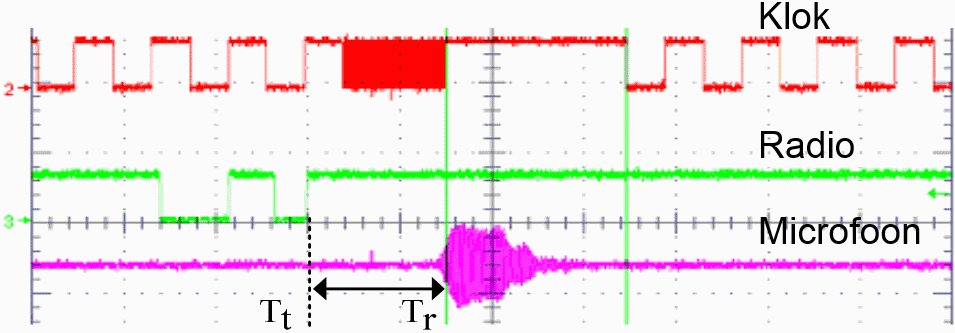
\includegraphics[width=0.7\textwidth]{tijdsdiagram.png}
    \caption{Tijdsdiagram radio en microfoon input. \textit{Bron: \cite{park2011beacon}}}
    \label{fig:tijdsdiagram}
\end{figure}

\section{Implementatie}\label{sec:implementatie}
De implementatie gebruikt de time of flight (TOF) om de afstand tussen beacons en de ontvanger te meten.

\subsection{Opstelling voor positiebepaling met hoogfrequent geluid}
De opstelling voor het bepalen van de positie bestaat uit vier bakens, die zijn genummerd van 0 tot 3. Elk baken bestaat uit een Arduino mini met daarop aangesloten een NRF2401L+-radio en een ultrasoon-zender. De bakens zijn bevestigd op een statief. De locaties van de bakens is bekend. Een voorbeeld van een opstelling met de vier bakens en een ontvanger is te zien in afbeelding~\ref{fig:opstelling}.

\begin{figure}[ht!]
    \centering
    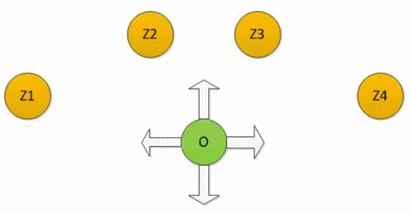
\includegraphics[width=0.7\textwidth]{opstelling.png}
    \caption{Opstelling met vier zenders en een ontvanger.}
    \label{fig:opstelling}
\end{figure}

De activiteiten van de verschillende bakens zijn als volgt: een van de bakens (Baken 0) verstuurt radioberichten met een interval van 100 ms. Dit bericht bestaat uit een uint8 (een getal tussen 0 en 255) waarin het nummer staat van de baken die aan de beurt is voor het versturen van een geluidspuls. (Baken 0 stuurt ook een bericht als baken 0 zelf aan de beurt is.) Als een baken een bericht ontvangt waarin zijn identificatienummer staat, verstuurt deze direct hierna een geluidspuls op een frequentie van circa 40kHz en met een duur van 50 ms. De bakens zijn dus nooit tegelijkertijd actief. Figuur~\ref{fig:tijdsdiagram_handleiding} toont de sequentie van activiteiten van de verschillende bakens. Verder zijn in tabel~\ref{table:instellingen} de verschillende instellingen te zien waarop de radio’s onderling communiceren.

\begin{figure}[ht!]
    \centering
    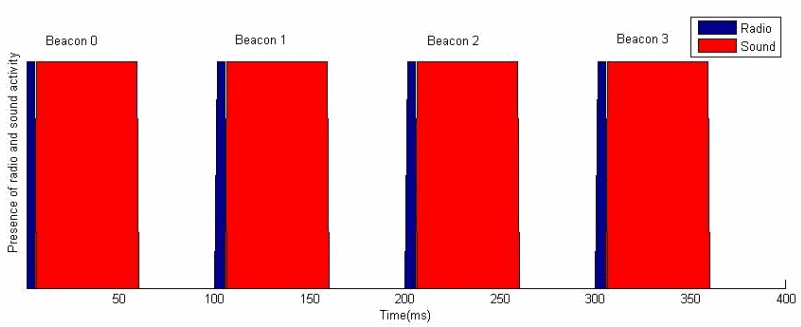
\includegraphics[width=0.7\textwidth]{tijdsdiagram_handleiding.png}
    \caption{Opstelling met vier zenders en een ontvanger.}
    \label{fig:tijdsdiagram_handleiding}
\end{figure}

\begin{table}[h]
    \begin{minipage}{\textwidth}
        \begin{tabular}{ l l }
            Kanaal                    & 76 (standaard RF24 instelling) \\
            Automatisch herverzenden  & Uit               \\
            Transmissiesnelheid       & 2 Mbps            \\
            Adres verzendende pipe    & 0xdeadbeefa1LL    \\
            Payload-grootte           & 1 byte
        \end{tabular}
        \caption{Instellingen radio}
        \label{table:instellingen}        
    \end{minipage}
\end{table}

\subsection{Algoritme}
Voor het omzetten van de afstanden tussen de ontvanger en de verschillende beacons zijn de berekeningen van Park et al.~\cite{park2011beacon} gebruikt. Doordat de afstanden tot de beacons bekend zijn kan een cirkel worden afgeleid waarop de ontvanger zich bevindt. Doordat meerdere cirkels bekend zijn kan de intersectie van die verschillende cirkels berekend worden: deze intersectie is de locatie van de ontvanger.

Er is gekozen voor deze berekening omdat de locaties van de beacons en de afstanden tot de beacons vrij intuitief als matrices gerepresenteerd worden. Als kanttekening moet vermeld worden dat dit algoritme niet alleen de x en y positie berekent, maar ook de z positie probeert te berekenen. Echter, omdat alle beacons op dezelfde hoogte staan is dit met onze opstelling niet mogelijk geweest. Er is immers niet te achterhalen of de z positie positief of negatief is; doordat alle beacons in een vlak staan kan de zco\"ordinaat gespiegeld worden. Vanwege deze reden hebben we ervoor gekozen om de z-co\"ordinaat niet in de resultaten op te nemen.

De gebruikte code is bijgevoegd in appendix~\ref{sec:code}. Merk op dat de posities van de beacons hardcoded is; deze kan worden aangepast indien de beacons een andere configuratie hebben. De positie van de ontvanger is relatief ten opzichte van de beacons.

Tijdens de tests is de lijn tussen beacon 1 en 2 als y-as gebruikt, en beacon 0 was op de x-as (die onder een hoek van 90 graden de y-as kruist). Het algoritme ondersteunt ook negatieve waardes voor als de ontvanger zich achter de y-as bevindt.

\section{Resultaten en discussie}\label{sec:resultaten}
\todo[inline]{bla}

\section{Conclusie}\label{sec:conclusie}
\todo[inline]{bla}

\bibliographystyle{plain}
\bibliography{verslag_week_5}

\newpage
\appendix
\section{Arduino code}
\label{sec:code}
% xxxxxxxxxxxxxxxxxxxxxxxxx Code Snippet STARTS xxxxxxxxxxxxxxxxxxxxxx
\lstset{
  language=C,                     % choose the language of the code
  stepnumber=1,                   % the step between two line-numbers. If it's 1, each line will be numbered
  basicstyle=\footnotesize,
 % numbersep=5pt,                 % how far the line-numbers are from the code
%  backgroundcolor=\color{white}, % choose the background color. You must add \usepackage{color}
  showspaces=false,               % show spaces adding particular underscores
  showstringspaces=false,         % underline spaces within strings
  showtabs=false,                 % show tabs within strings adding particular underscores
  tabsize=4,                      % sets default tabsize to 2 spaces
  captionpos=t,                   % sets the caption-position to top
  breaklines=true,                % sets automatic line breaking
  breakatwhitespace=true,         % sets if automatic breaks should only happen at whitespace
 % title=\lstname,                % show the filename of files included with \lstinputlisting;
 % identifierstyle=\color{identifierColor},
 % caption={Array of Pointers to Strings},
 % frame=lrtb,
 % keywordstyle=\color{purple},         % keyword style
 % commentstyle=\color{blue},           % comment style
 % stringstyle=\color{violet},          % string literal style
 belowcaptionskip = 0.2in,            % Space below caption
 abovecaptionskip = 0.2in             % Space above caption
}
% \lstset{language=C}
\begin{lstlisting}
/*
    Positioning system for Arduino One with RF24 radio chip
*/
#include <SPI.h>
#include "nRF24L01.h"
#include "RF24.h"
#include "printf.h"
#include "MatrixMath.h"

#define N (3)
// Kunstmatige waarde voor Z coordinaten
#define Z 1.0
// Percentage verschil (0 < MAX_DIFF <= 1) dat tussen twee metingen mag zitten.
#define MAX_DIFF (0.25)
// Percentage dat de nieuwste meting in het gemiddelde meetelt (0 < WEIGHT <= 1)
// Bij WEIGHT=1 wordt er geen gemiddelde bijgehouden, maar is de nieuwste meting de enige die meetelt.
#define WEIGHT (0.2)

RF24 radio(3, 9);
unsigned long radiotime;
unsigned long audiotime;
unsigned long timelimit = 50000LL;
uint8_t activeBeacon;

float pos[4][2] = { // Positions van de beacons; pos[1][1] is de y positie van beacon 1
    {0.0, 75.0},
    {72.0, 0.0},
    {294.0, 0.0},
    {372.0, 136.0}
};

float D[4];


void setup() {
  // initialize the serial communication:
  Serial.begin(9600);
  printf_begin();

  // Setup and configure rf radio
  radio.begin();
  radio.setRetries(0,0);

  radio.setDataRate(RF24_2MBPS);
  radio.setChannel(76);
  radio.setPayloadSize(1);
  radio.openReadingPipe(1, 0xdeadbeefa1LL);
  radio.openWritingPipe(0xdeadbeefa1LL);
  radio.startListening();
  radio.setAutoAck(false);
}

void loop() {
  while(radio.available()) { 
    radio.read(&activeBeacon, sizeof(uint8_t)); 
  }
  while (! radio.available());

  radiotime = micros();
  radio.read( &activeBeacon, sizeof(uint8_t));

  if(activeBeacon > 3) { return; }

  while(analogRead(A0) < 50) {
    audiotime = micros();
    if(audiotime - radiotime > timelimit) {
      return; 
    }
  }
  
  float diff = audiotime - radiotime;
  diff = diff * 0.03432; // Afstand tot beacon in cm

  //Zwak uitschieters een beetje af: max 30% increase
  if(diff > (D[activeBeacon]* (1.0 + MAX_DIFF)) && D[activeBeacon] > 0) {
    diff = D[activeBeacon] * (1.0 + MAX_DIFF);
  }
  
  if(diff < (D[activeBeacon]* (1.0 - MAX_DIFF))) {
    diff = D[activeBeacon]*(1.0 - MAX_DIFF);
  }
  
  D[activeBeacon] = D[activeBeacon]*(1.0 - WEIGHT) + diff*WEIGHT; // Weer schuivend gemiddelde */
  //D[activeBeacon] = diff;

  if(activeBeacon == 3) {
    calcPosition();
  }
}

float A[N][N];
float B[N];

void calcPosition() {
    // Relatieve afstanden tussen de nodes; gebruikt node 3 nog niet!
    A[0][0] = 2*pos[1][0] - 2*pos[0][0]; A[0][1] = 2*pos[1][1] - 2*pos[0][1]; A[0][2] = Z;
    A[1][0] = 2*pos[2][0] - 2*pos[1][0]; A[1][1] = 2*pos[2][1] - 2*pos[1][1]; A[1][2] = Z;
    A[2][0] = 2*pos[0][0] - 2*pos[2][0]; A[2][1] = 2*pos[0][1] - 2*pos[2][1]; A[2][2] = Z;
    Matrix.Invert((float*)A,N);

    B[0] = (D[0]*D[0]) - (D[1]*D[1]) - (pos[0][0]*pos[0][0]) + (pos[1][0]*pos[1][0]) - (pos[0][1]*pos[0][1]) + (pos[1][1]*pos[1][1]);
    B[1] = (D[1]*D[1]) - (D[2]*D[2]) - (pos[1][0]*pos[1][0]) + (pos[2][0]*pos[2][0]) - (pos[1][1]*pos[1][1]) + (pos[2][1]*pos[2][1]);
    B[2] = (D[2]*D[2]) - (D[0]*D[0]) - (pos[2][0]*pos[2][0]) + (pos[0][0]*pos[0][0]) - (pos[2][1]*pos[2][1]) + (pos[0][1]*pos[0][1]);
    
    float P3[N];
    Matrix.Multiply((float*)A,(float*)B,N,N,1,(float*)P3);
    printf("Position (P3): (%d,%d)\n", (int) P3[0], (int) P3[1]);
    

    // Relatieve afstanden tussen de nodes; gebruikt node 2 nog niet!
    A[0][0] = 2*pos[1][0] - 2*pos[0][0]; A[0][1] = 2*pos[1][1] - 2*pos[0][1]; A[0][2] = Z;
    A[1][0] = 2*pos[3][0] - 2*pos[1][0]; A[1][1] = 2*pos[3][1] - 2*pos[1][1]; A[1][2] = Z;
    A[2][0] = 2*pos[0][0] - 2*pos[3][0]; A[2][1] = 2*pos[0][1] - 2*pos[3][1]; A[2][2] = Z;
    Matrix.Invert((float*)A,N);

    B[0] = (D[0]*D[0]) - (D[1]*D[1]) - (pos[0][0]*pos[0][0]) + (pos[1][0]*pos[1][0]) - (pos[0][1]*pos[0][1]) + (pos[1][1]*pos[1][1]);
    B[1] = (D[1]*D[1]) - (D[3]*D[3]) - (pos[1][0]*pos[1][0]) + (pos[3][0]*pos[3][0]) - (pos[1][1]*pos[1][1]) + (pos[3][1]*pos[3][1]);
    B[2] = (D[3]*D[3]) - (D[0]*D[0]) - (pos[3][0]*pos[3][0]) + (pos[0][0]*pos[0][0]) - (pos[3][1]*pos[3][1]) + (pos[0][1]*pos[0][1]);
    float P2[N];
    Matrix.Multiply((float*)A,(float*)B,N,N,1,(float*)P2);
    printf("Position (P2): (%d,%d)\n", (int) P2[0], (int) P2[1]);
    
    
    // Relatieve afstanden tussen de nodes; gebruikt node 1 nog niet!
    A[0][0] = 2*pos[2][0] - 2*pos[0][0]; A[0][1] = 2*pos[2][1] - 2*pos[0][1]; A[0][2] = Z;
    A[1][0] = 2*pos[3][0] - 2*pos[2][0]; A[1][1] = 2*pos[3][1] - 2*pos[2][1]; A[1][2] = Z;
    A[2][0] = 2*pos[0][0] - 2*pos[3][0]; A[2][1] = 2*pos[0][1] - 2*pos[3][1]; A[2][2] = Z;
    Matrix.Invert((float*)A,N);
   
    B[0] = (D[0]*D[0]) - (D[2]*D[2]) - (pos[0][0]*pos[0][0]) + (pos[2][0]*pos[2][0]) - (pos[0][1]*pos[0][1]) + (pos[2][1]*pos[2][1]);
    B[1] = (D[2]*D[2]) - (D[3]*D[3]) - (pos[2][0]*pos[2][0]) + (pos[3][0]*pos[3][0]) - (pos[2][1]*pos[2][1]) + (pos[3][1]*pos[3][1]);
    B[2] = (D[3]*D[3]) - (D[0]*D[0]) - (pos[3][0]*pos[3][0]) + (pos[0][0]*pos[0][0]) - (pos[3][1]*pos[3][1]) + (pos[0][1]*pos[0][1]);
    float P1[N];
    Matrix.Multiply((float*)A,(float*)B,N,N,1,(float*)P1);
    printf("Position (P1): (%d,%d)\n", (int) P1[0], (int) P1[1]);
    
    
    // Relatieve afstanden tussen de nodes; gebruikt node 0 nog niet!
    A[0][0] = 2*pos[2][0] - 2*pos[1][0]; A[0][1] = 2*pos[2][1] - 2*pos[1][1]; A[0][2] = Z;
    A[1][0] = 2*pos[3][0] - 2*pos[2][0]; A[1][1] = 2*pos[3][1] - 2*pos[2][1]; A[1][2] = Z;
    A[2][0] = 2*pos[1][0] - 2*pos[3][0]; A[2][1] = 2*pos[1][1] - 2*pos[3][1]; A[2][2] = Z;
    Matrix.Invert((float*)A,N);
   
    B[0] = (D[1]*D[1]) - (D[2]*D[2]) - (pos[1][0]*pos[1][0]) + (pos[2][0]*pos[2][0]) - (pos[1][1]*pos[1][1]) + (pos[2][1]*pos[2][1]);
    B[1] = (D[2]*D[2]) - (D[3]*D[3]) - (pos[2][0]*pos[2][0]) + (pos[3][0]*pos[3][0]) - (pos[2][1]*pos[2][1]) + (pos[3][1]*pos[3][1]);
    B[2] = (D[3]*D[3]) - (D[1]*D[1]) - (pos[3][0]*pos[3][0]) + (pos[1][0]*pos[1][0]) - (pos[3][1]*pos[3][1]) + (pos[1][1]*pos[1][1]);
    float P0[N];
    Matrix.Multiply((float*)A,(float*)B,N,N,1,(float*)P0);
    printf("Position (P0): (%d,%d)\n", (int) P0[0], (int) P0[1]);
    
    // Bereken het gemiddelde van de verschillende metingen:
    int avg[N];
    avg[0] = (int) (P0[0] + P1[0] + P2[0] + P3[0]) / 4.0;
    avg[1] = (int) (P0[1] + P1[1] + P2[1] + P3[1]) / 4.0;
    avg[2] = (int) (P0[2] + P1[2] + P2[2] + P3[2]) / 4.0;
  
    printf("Position: (%d,%d)\n\n", avg[0], avg[1]);
}
\end{lstlisting}

\end{document}
